\documentclass[letter,french]{report}
\usepackage[T1]{fontenc}
\usepackage[utf8]{inputenc} 
\usepackage{lmodern}
\usepackage{babel}
\usepackage[pdftex]{graphicx}
\usepackage[nointegrals]{wasysym}
\usepackage{amsmath,amssymb}


\begin{document}
	\title{Devoir 2 IFT 3913}
	\author{Ludovic André et Gevrai Jodoin-Tremblay}
	\date{Remis le 2 Novembre 2017}
	\maketitle
	
	
  \section*{Introduction}

	\subsection*{Description du logiciel}
	Ce logiciel affiche une interface usager simple, très semblable
	à l'exemple d'interface usager de l'énoncé du travail pratique. Le bouton "Charger
	fichier" ouvre une fenêtre système permettant de sélectionner un fichier .ucd.
	Lorsqu'un fichier est choisi, il est \emph{parser} et ses éléments sont affichés dans
	les champs correspondants de l'interface. L'usager peut selectionner les
  différents éléments de l'interface pour avoir plus de détails sur ceux-ci.

  Aussi, en sélectionnant une classe dans la boîte de gauche, le programme
  affiche toutes les métriques pour cette classe dans la boîte de droite. Il est
  aussi possible d'afficher la définition d'une métriques dans la boîte de
  détails simplement en la sélectionnant.
  
  Il y a certaines métriques qui peuvent retourner une valeur négative qui vaut -1. Ces métriques en questions sont DIT,CLD et NOD. Cela veut dire que lors du calcul le système a détecté qu'une classe "A" à un enfant classe "B" et cette Classe "B" à un enfant "A". À ce moment, les métriques sont automatiquement mises à -1, car il ne peut pas dire avec certitudes s’il se situe à la racine ou à la feuille.

  Finalement, l'utilisateur peut exporter les métriques du modèle courant en
  appuyant sur le bouton \emph{Exporter métriques}. Une boîte de dialogue
  permetera ainsi de sélectionner la destination et un fichier \emph{.csv} sera
  créé contenant le résultat de toutes les métriques pour chaque classe.

  \subsection*{Arborescence de l'archive}
	\subsubsection*{makefile}
	Nous avons opté pour un \emph{makefile} histoire de rendre la compilation et l'exécution
	la plus facile possible sur les machines du DIRO. Un simple \emph{make} compile
	l'entièreté du logiciel et l'exécute. Pour voir les autres options, \emph{make help}
	explique les différentes commandes possibles.

	\subsubsection*{src}
  Contient tous le code du projet, sans exception. Puisque nous n'avons utilisé
  aucune librairie externe dans le projet, l'entièreté du code source s'y trouve.
  La seule librairie externe utilisée est en effet \emph{JUnit}, mais le code
  pour les tests est séparé du code source du projet.

  La fonction \emph{main} de notre programme se trouve dans la classe
  \emph{App.java}, que nous avons gardé la plus minimale possible.

  Évidemment, l'arborescence de ce fichier suit l'arborescence de paquet de
  notre code que l'on avait présenté en grande partie dans le rapport du TP1.

	\subsubsection*{\_build}
  Histoire de garder notre dossier src assez propre, la compilation des fichiers
  \emph{.class} se fait vers ce dossier.

	\subsubsection*{rapport}
  Tout simplement toutes les ressources nécessaires à l'impression de ce
  merveilleux rapport!

  \subsubsection*{tests}
  Tout le nécessaire pour rouler notre batterie de test grâce à \emph{JUnit}. Il
  est primordial de ne rien modifier dans ce dossier pour garantir la validité
  de nos tests.
	
	\section*{Conception}

  \subsection*{Modifications depuis version 1}

  La grande majorité de notre \emph{backend} n'a pas été modifié, nous avons
  simplement ajouté les métriques. En effet, le
  paquet \emph{uml}, dont on avait donné le diagramme de classe dans le rapport
  du TP1, n'a subi aucun changement.

  Le pattern MVC étant très modulaire, nous avons pû simplement ajouter les
  éléments nécessaires au controlleur et à l'interface sans vraies embûches.
	
	\subsection*{Ajout des métriques}
  Puisque nous avions fait attention d'appliquer au meilleur de nos
  connaissances, les \emph{patterns} de conception orienté-objet, notre code
  était assez facile à étendre avec des nouvelles fonctionalités. En effet, pour
  représenter les calculs de métriques, nous avons créé une classe abstraite
  \emph{BaseMetric} contenant tous les attributs et méthodes communes à toutes
  les métriques, avec la seule méthode abstraite
  \texttt{compute(UMLModel,UMLClass)}. Cette méthode, qui doit être défini par
  les sous-classes, est évidemment le calcul de la métrique en particulier.
  Cette hiérarchie permet de facilement ajouter de nouvelles métriques en ne
  définissant que les parties importantes de celle-ci.
  \begin{center}
	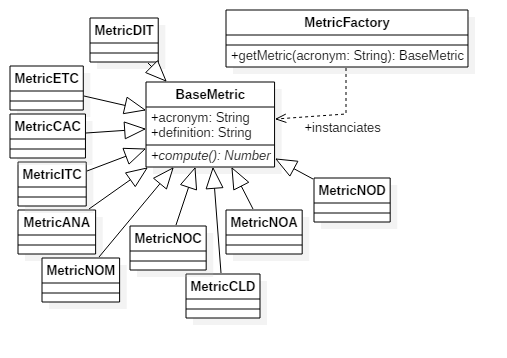
\includegraphics[scale=.6]{images/Metrics_diagram.png}
  \end{center}

  Aussi, comme on peut souvent le voir avec ce genre d'arbre de classe, une
  classe \emph{MetricFactory} est utilisée pour instancier une métrique en
  particulier, simplement avec son acronyme.

  Ces métriques sont tous simplement utilisées par le controlleur principal
  sur le modèle \emph{UML} chargé dans le programme. Il est à noter que le
  paquet \emph{uml} n'a aucune connaissance des métriques.
	
	\section*{Implantation}
	
	\subsection*{Parseur}
  Nous avons réglé l'erreur de \emph{parsing} causé par un fichier vide en
  entrée. On affiche maintenant une petite fenêtre signalant à l'utilisateur que
  le fichier d'entrée était vide. Par le fait même, les fichiers \emph{.ucd}
  erronées affiches maintenant aussi cette fenêtre, avec un message approprié.
	
	\subsection*{MVC}
  Ce patron s'est avéré être un excellent choix initial pour notre implantation.
  Les ajouts apportés au code pour les nouvelles fonctionnalités étaient isolés
  du code déjà existants. Il ne suffisait que d'ajouter quelques fonctions et
  \emph{Listeners} au controlleur pour les implémenter.
	
	\section*{Tests}
  Pour faciliter la création et l'exécution de notre suite de tests, nous avons opté pour
  l'écriture de tests automatisés grâce à la librairie bien connue \emph{JUnit}.
  L'immense avantage de cette approche est d'éliminer la lourde tâche
  d'effectuer des tests manuels à chaque fois que l'on effectue un changement
  dans le code. Aussi, puisque nous avions déjà les résultats de certaines
  métriques, un de nous a écrit les tests pendant que l'autre implémentait les
  dites métriques. On pourrait dire que cette méthode de travail est favorable
  car celui qui écrit les tests n'est pas biaisé par son propre travail.

  Il est a noté que lorsque l'on compile avec la commande \texttt{make all}, la
  compilation ne réussira pas si un ou plusieurs tests échouent. 

  \subsection*{Parseur}
  Le fichier \emph{ParserTest.java} teste notre parseur avec tous les fichiers
  offerts par le démonstrateur, et notre programme passe tous ces tests. Nous
  avons aussi ajouté quelques tests personnels, soit \emph{BadFile.ucd} qui est
  simplement un exemple de fichier invalide devant retourner une erreur dans le
  parseur, ainsi que \emph{LeagueMetriques.ucd} permettant de mieux tester
  certaines métriques.

  Tous ces fichiers passe correctement nos tests.

  \subsection*{Métriques}
  Les fichier \emph{MetricsTestX.java} testent le calcul des métriques sur trois
  fichiers en entrée, et la Table 1 donne les sorties prévues de chacun pour
  chaque métrique.
 
  \begin{table}[]
    \centering
    
    \caption{Valeurs espérées des métriques pour les tests}
    \begin{tabular}{lccccc}
      Metrique&\begin{tabular}[c]{@{}c@{}}League.ucd\\ Equipe\end{tabular} & \begin{tabular}[c]{@{}c@{}}LeagueMetriques1.ucd\\ Equipe\end{tabular} & \begin{tabular}[c]{@{}c@{}}LeagueMetriques1.ucd\\ Joueur\end{tabular} &  \\
      ANA & 0.33                & 0.33                          & 0                            \\
      NOM & 3                   & 4                             & 4                            \\
      NOA & 1                   & 3                             & 3                            \\
      ITC & 1                   & 1                             & 0                            \\
      ETC & 1                   & 1                             & 2                            \\
      CAC & 3                   & 0                             & 0                            \\
      DIT & 0                   & 3                             & 1                            \\
      CLD & 0                   & 0                             & 2                            \\
      NOC & 0                   & 0                             & 1                            \\
      NOD & 0                   & 0                             & 2                                       
    \end{tabular}
  \end{table}


\
\begin{table}
	\centering
	
	\caption{Valeurs espérées des métriques pour les tests}
	\begin{tabular}{lccccc}
		  Metrique&\begin{tabular}[c]{@{}c@{}}LeagueMetriques2.ucd\\ Equipe\end{tabular}&
		 \begin{tabular} [c]{@{}c@{}}StadeBoucle.ucd\\ Equipe\end{tabular} \\
		 
		 ANA   & 0.33         & 0.33             \\
		 NOM   & 3            & 4                \\
		 NOA   & 3            & 3                \\
		 ITC   & 1            & 1                \\
		 ETC   & 2            & 1                \\
		 CAC   & 3            & 0                \\
		 DIT   & 1            & -1               \\
		 CLD   & 0            & -1               \\
		 NOC   & 0            & 1                \\
		 NOD   & 0            & -1               
	\end{tabular}		 
\end{table}

\subsubsection*{Problème}
Lors de l'implémentation des métriques DIT,CLD et NOD, nous nous sommes heurtés à un cas extrême. Pour ces 3 métriques, nous devons faire une recherche itérative pour savoir le nombre de sous-causes directes et indirectes(NOD), le chemin le plus long entre une classe x et sa racine et le chemin le plus long entre la classe x et sa feuille la plus basse. Dans ces 3 cas, le problème se situe si on a une boucle dans les généralisations. Si une classe "A" a comme enfant une classe "B" et la classe "B" a comme enfant la classe "A", on a une boucle. Cela a causé une boucle infinie pour ces métriques.On peut le voir avec le fichier \emph{StadeBoucle.ucd} Pour remédier à ce problème ,nous avons ajouté une condition de vérification de boucle dans notre arbre de généralisation. Lorsqu'il détecte cette boucle de généralisation, il va mettre ces trois métriques à -1 pour signifié qu'il y a un problème dans notre graphe UCD. 

  \subsection*{Interface}
  Malheureusement, il est très difficile, voire impossible, de tester
  automatiquement une interface graphique, c'est pourquoi cette section
  contient quelques tests manuels.

  \subsubsection*{Fichier valide - League.ucd}
  - Fichier en entrée : League.ucd
  - Sortie prévue : 

  

	\section*{Développements futur}
	Il serait très utile de pouvoir modifier un modèle UML directement à partir de l'interface,
	et permettre l'exportation du modèle ainsi modifier vers un fichier /.ucd/. Aussi, lorsque l'on détecte un cas problématique d'une boucle à l'infinie pour la généralisation des classes. Il serait intéressant d'afficher un message indiquant qu'il y a un problème avec la généralisation et de retravailler cette section, car on a une boucle. 
	
	
\end{document}
